\documentclass[12pt,oneside]{exam}

% This package simply sets the margins to be 1 inch.
\usepackage[margin=1in]{geometry}

% These packages include nice commands from AMS-LaTeX
\usepackage{amssymb,amsmath,amsthm,amsfonts,latexsym,verbatim,xspace,setspace}
\usepackage{hyperref}
\usepackage{graphicx}

% Make the space between lines slightly more
% generous than normal single spacing, but compensate
% so that the spacing between rows of matrices still
% looks normal.  Note that 1.1=1/.9090909...
\renewcommand{\baselinestretch}{1.1}
\renewcommand{\arraystretch}{.91}

% Define environments for exercises.
\newenvironment{exercise}[1]{\vspace{.1in}\noindent\textbf{Exercise #1 \hspace{.05em}}}{}
\newenvironment{newsolution}{\vspace{.1in}\noindent\textbf{Solution: \hspace{.05em}}}{}

% define shortcut commands for commonly used symbols
\newcommand{\R}{\mathbb{R}}
\newcommand{\C}{\mathbb{C}}
\newcommand{\Z}{\mathbb{Z}}
\newcommand{\Q}{\mathbb{Q}}
\newcommand{\N}{\mathbb{N}}
\newcommand{\calP}{\mathcal{P}}
\DeclareMathOperator{\sech}{sech}
\DeclareMathOperator{\csch}{csch}
\DeclareMathOperator{\vsspan}{span}

\title{Math 203 - Summer I 2020: Solutions to Homework 3}

%%%%%%%%%%%%%%%%%%%%%%%%%%%%%%%%%%%%%%%%%%

\begin{document}

\begin{flushright}
\sc MAT 203 - Summer I 2020\\
July 2, 2020
\end{flushright}
\bigskip
 
\begin{center}
\textsf{Homework 4 solutions} 
\end{center}

%%%%%%%%%%%%%%%%%%%%%%%%%%%%%%%%%%%%%%%%

\begin{exercise}{1}
Evaluate the triple iterated integral
\begin{equation*}
\int_{0}^{1}\int_{0}^{1+\sqrt{y}}\int_{0}^{xy} y \, dz \, dx \, dy.
\end{equation*}
\end{exercise}

\begin{newsolution} 
\begin{align*}
\int_{0}^{1} \int_{0}^{1+\sqrt{y}} \int_{0}^{xy} y \, dz \, dx \, dy & = \int_{0}^{1} \int_{0}^{1+\sqrt{y}} \left[ yz\Big|_{z=0}^{z=xy} \right] \, dx\, dy \\
& = \int_{0}^{1} \int_{0}^{1+\sqrt{y}} xy^2 \, dx \, dy \\
& = \int_{0}^{1} \left[ \frac{x^2y^2}{2} \Big|_{x=0}^{x=1+\sqrt{y}} \right] \, dy \\
& = \int_{0}^{1} \frac{(1+\sqrt{y})^2 y^2}{2} \, dy \\
& = \int_{0}^{1} \frac{(1+2\sqrt{y}+y) y^2}{2} \, dy \\
& = \int_{0}^{1} \frac{y^2}{2} + y^{\frac{5}{2}} + \frac{y^3}{2} \, dy \\
& = \left[ \frac{y^3}{6} + \frac{2}{7}y^{\frac{7}{2}} + \frac{y^4}{8} \Big|_{y=0}^{y=1} \right] \\
& = \frac{1}{6} + \frac{2}{7} + \frac{1}{8} \\
& = \frac{97}{168}
\end{align*}
\end{newsolution}

\begin{exercise}{2}
Sketch the solid whose volume is given by the iterated integral. Rewrite the integral using the order $$dy dx dz$$ (do not evaluate the integral in either order). 
\begin{equation*}
\int_{0}^{6} \int_{0}^{6-x} \int_{0}^{6-x-y} dz dy dx
\end{equation*}
\end{exercise}

\begin{newsolution}
The region of integration is the tetrahedron sketched below. 
\begin{center}
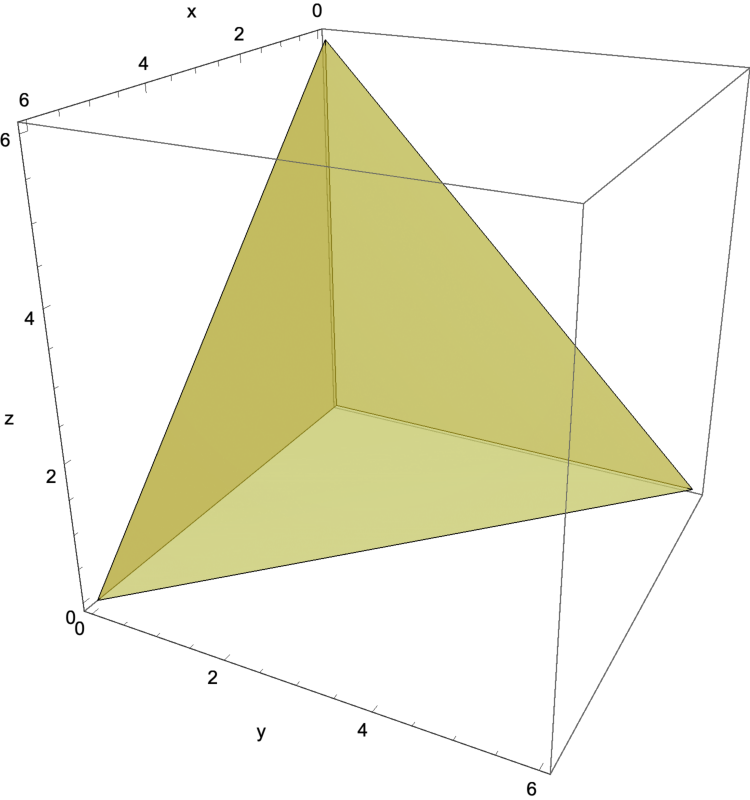
\includegraphics[scale=0.5]{p9.pdf}
\end{center}
We seek to describe volume of the solid by means of integration with respect to the order $dy \, dx \, dz$. That is, we consider $z$ as an independent variable, $x$ as depending upon $z$, and $y$ depending on both $x$ and $z$. The range of values that $z$ can attain within this solid is $0 \leq z \leq 6$. For a fixed value of $z$, the lower bounds for $x$ and $y$ are constants, $x_{\mathrm{lower}}=0$, $y_{\mathrm{lower}}=0$. The upper bound for $x$ is attained when $y$ is at its minimum, $y=0$. By means of the equation of the plane bounding the tetrahedron, 
\begin{equation*}
x_{\mathrm{upper}} + 0 + z = 6 \Rightarrow x_{\mathrm{upper}} = 6-z.
\end{equation*}
For fixed $x$ and $z$, the upper limit of integration relative to $y$ can be found analogously, 
\begin{equation*}
x + y_{\mathrm{upper}}  + z = 6 \Rightarrow y_{\mathrm{upper}} = 6-x-z.
\end{equation*}
The integral can thus be rewritten as 
\begin{equation*}
\int_{0}^{6} \int_{0}^{6-z} \int_{0}^{6-x-z} \, dy \, dx \, dz.
\end{equation*}
\end{newsolution}


\begin{exercise}{3}
Use cylindrical coordinates to find the volume of the solid bounded above by 
\begin{equation*}
3x^2+3y^2+z^2 = 45,
\end{equation*}
and below by the xy-plane.
\end{exercise}

\begin{newsolution}
Below is a plot of the region of integration.
\begin{center}
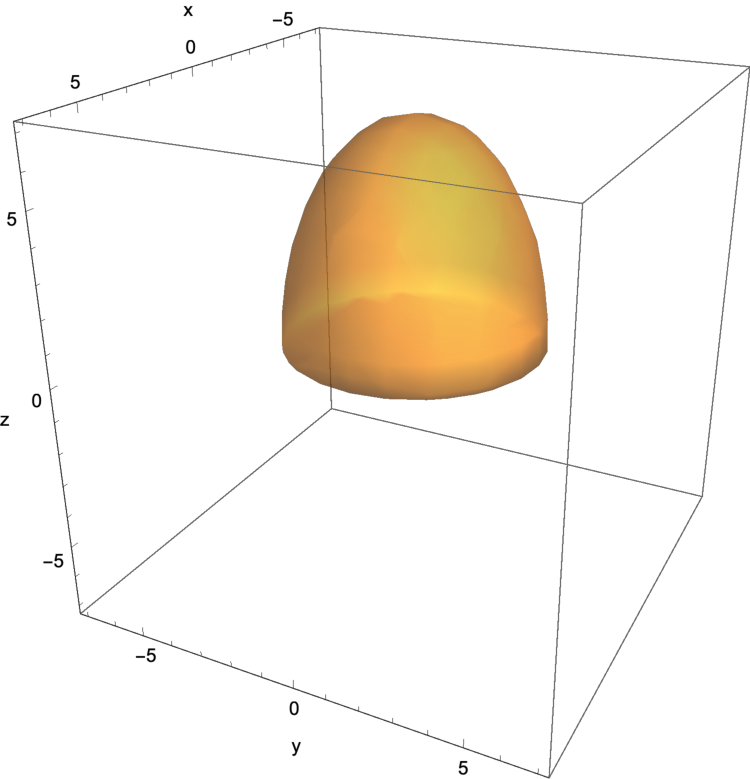
\includegraphics[scale=0.5]{p10.pdf}
\end{center}
We will use the angular variable $\theta$ as independent variable, $0 \leq \theta \leq 2\pi$. We also choose $z$ as our intermediate variable of integration. As it turns out, the range of values for $0$ does not depend on the angle $\theta$, $0 \leq z \leq \sqrt{45}=3\sqrt{5}$. Finally, we turn to the axial radius $r$, whose range of values depends upon the height $z$. At its maximum, $r$ is linked to $z$ by the equation of the ellipsoid, 
\begin{equation*}
3r_{\mathrm{upper}}^{2} +z^2 =45 \Rightarrow r_{upper} = \sqrt{\frac{45-z^2}{3}}
\end{equation*}
The volume can be computed in cylindrical coordiantes as follows:
\begin{align*}
V & = \int_{0}^{2\pi} \int_{0}^{3\sqrt{5}} \int_{0}^{\sqrt{\frac{45-z^2}{3}}} r \, dr \, dz \, d\theta \\
& = \int_{0}^{2\pi} \int_{0}^{3\sqrt{5}} \left[ \frac{r^2}{2} \Big|_{r=0}^{r=\sqrt{\frac{45-z^2}{3}}} \right] \, dz \,d\theta \\
& = \int_{0}^{2\pi} \int_{0}^{3\sqrt{5}}\frac{45-z^2}{6} \, dz \, d\theta \\
& = \int_{0}^{2\pi}  \left[ \frac{15z}{2} - \frac{z^3}{18} \Big|_{z=0}^{z=3\sqrt{5}} \right] \, d\theta \\
& =  \int_{0}^{2\pi} 15\sqrt{5}  \, d\theta \\
& = 30\pi\sqrt{5}
\end{align*}
\end{newsolution} 

\begin{exercise}{4}
Use spherical coordinates to find the volume of the solid bounded above by 
\begin{equation*}
x^2+y^2+z^2=36,
\end{equation*}
and below by
\begin{equation*}
z=\sqrt{x^2+y^2}.
\end{equation*}
\end{exercise}

\begin{newsolution}
Below is a plot of the region of integration.
\begin{center}
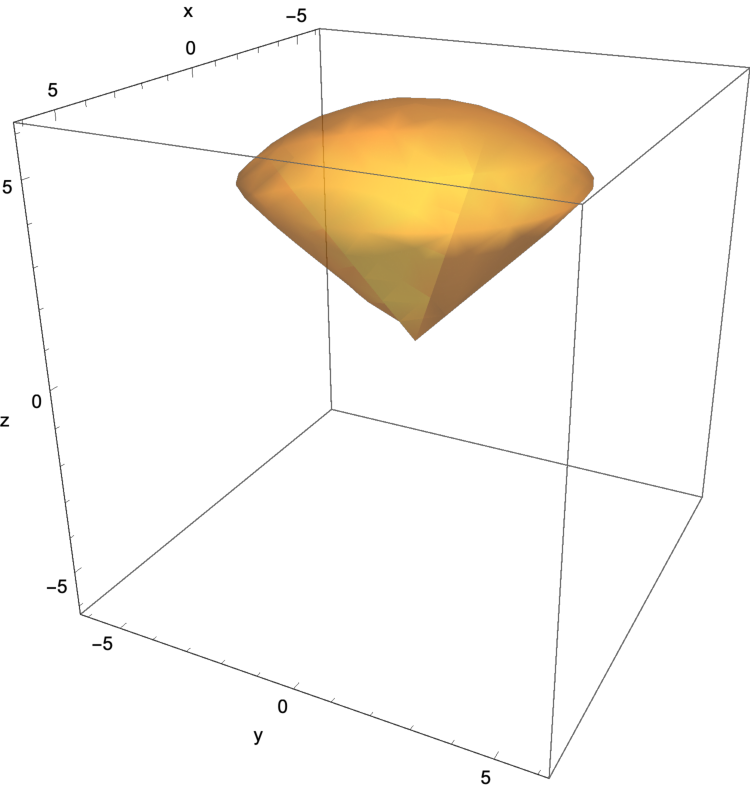
\includegraphics[scale=0.5]{p11.pdf}
\end{center}
We will choose the radius (distance to origin) as the independent variable, identifying the bounds as $r_{\mathrm{lower}}=0$ and $r_{\mathrm{upper}}=6$ (the radius of the sphere). The bounds for longitude angle $\theta$ are independent of $r$, $\theta_{\mathrm{lower}}=0, \theta_{\mathrm{upper}}=2\pi$. To understand the range of values for the latitude angle we project this plot onto the $zy$-plane ($x=0$). Below is a projection of the bounding surfaces.
\begin{center}
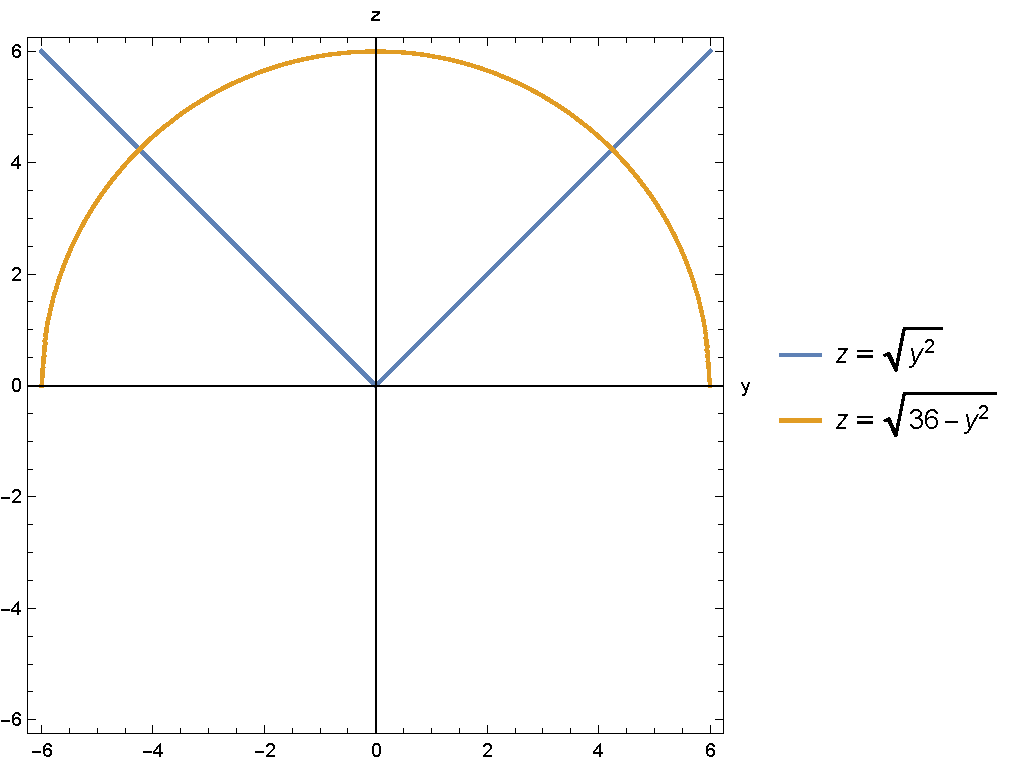
\includegraphics[scale=0.5]{p12.pdf}
\end{center}
The intersection points occur when
\begin{equation*}
y^2 = 36-y^2 \Rightarrow y^2 = 18,
\end{equation*}
thus the corresponding value of $z$ is $z=3\sqrt{2}$. Using the relation between Cartesian and spherical coordinates, we find the angle of intersection
\begin{align*}
z & = r\cos(\phi) \\
3\sqrt{2} & = 6\cos(\phi) \\
\frac{\sqrt{2}}{2} & = \cos(\phi) \\
\frac{\pi}{4} & = \phi.
\end{align*} 
Thus we compute the volume in spherical coordinates as 
\begin{align*}
V & = \int_{0}^{6} \int_{0}^{2\pi} \int_{0}^{\frac{\pi}{4}} r^2\sin(\phi) \, d\phi \, d\theta \, dr \\
& = \int_{0}^{6} \int_{0}^{2\pi} \left[ -r^2\cos(\phi) \Big|_{\phi =0}^{\phi = \frac{\pi}{4}} \right] \, d\theta \, dr\\
& = \int_{0}^{6} \int_{0}^{2\pi} \frac{r^2(2-\sqrt{2})}{2} \, d\theta \, dr \\
& = \int_{0}^{6} r^2(2-\sqrt{2})\pi \, dr \\
& = \left[ \frac{r^3(2-\sqrt{2})\pi}{3} \Big|_{r=0}^{r=6} \right] \\
& = 72(2-\sqrt{2})\pi.
\end{align*}
\end{newsolution}

\begin{exercise}{5}
Use the change of variables
\begin{equation*}
x = \frac{u+v}{4}, y=\frac{v-u}{2}
\end{equation*}
to evaluate the integral 
\begin{equation*}
\int\int_{R} 16xy \, dA,
\end{equation*}
where $R$ is the parallelogram with vertices $(0,2),(1,0),(1,4),(2,2)$.
\end{exercise}

\begin{newsolution}
Below is a plot of the region of integration.
\begin{center}
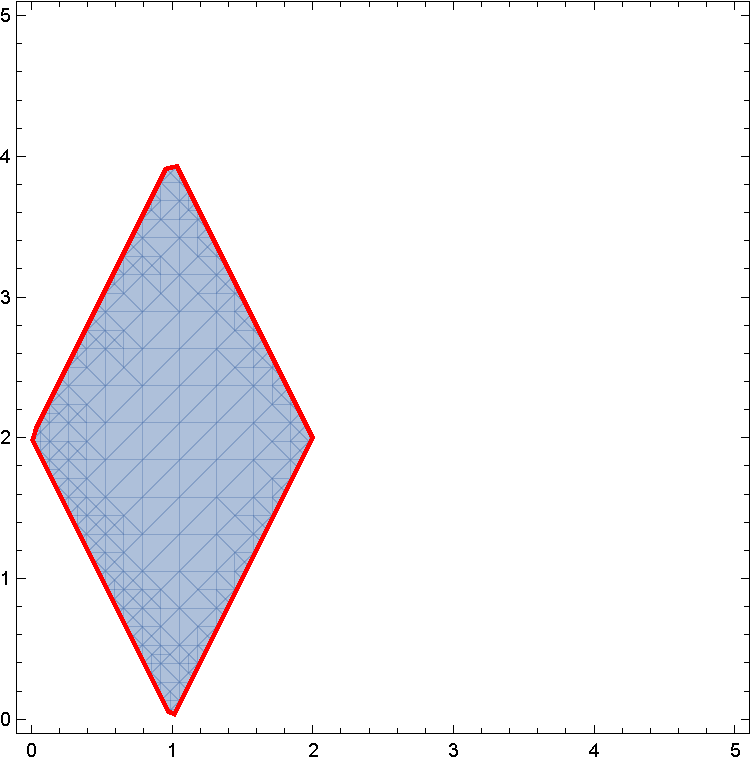
\includegraphics[scale=0.5]{p13.pdf}
\end{center}
The boundary curves are described by the following equations, 
\begin{align*}
2x-y & = -2, \\
2x-y & = 2, \\
2x + y & = 2, \\
2x+y & = 6.
\end{align*}
The equations relating $x,y$ to $u,v$ may be rewritten as 
\begin{equation*}
u  = 2x-y, \, \, v  = 2x+y,
\end{equation*}
whereas the relation between the area elements is
\begin{equation*}
dA = dx \, dy = \frac{1}{4} du \, dv.
\end{equation*}
We may thus calculate the integral in terms of the new coordinates as 
\begin{align*}
\int \int_{R} 16xy \, dA & = \int_{2}^{6}\int_{-2}^{2}  16\left(\frac{u+v}{4}\right)\left(\frac{v-u}{2}\right) \frac{1}{4} \, du \, dv \\
& = \int_{2}^{6} \int_{-2}^{2}  \frac{v^2-u^2}{2} \, du \, dv \\
& = \int_{2}^{6} \left[ \frac{uv^2}{2} - \frac{u^3}{6} \Big|_{u=-2}^{u=2} \right] \, dv \\
& = \int_{2}^{6} -\frac{8}{3} + 2v^2 \, dv \\
& = \left[-\frac{8v}{3} + \frac{2v^3}{3} \Big|_{v=2}^{v=6} \right] \\
& = 128.
\end{align*}
\end{newsolution}. 

\begin{exercise}{6}
Use the change of variables 
\begin{equation*}
x =u, y = \frac{v}{u}
\end{equation*}
to evaluate the integral 
\begin{equation*}
\int\int_{R} \frac{x}{1+x^2y^2} dA
\end{equation*}
where $$R$$ is the region bounded by the curves 
\begin{equation*}
x=1, x=5, xy=1, xy=5.
\end{equation*}
\end{exercise}

\begin{newsolution}
Below is a plot of the region of integration.
\begin{center}
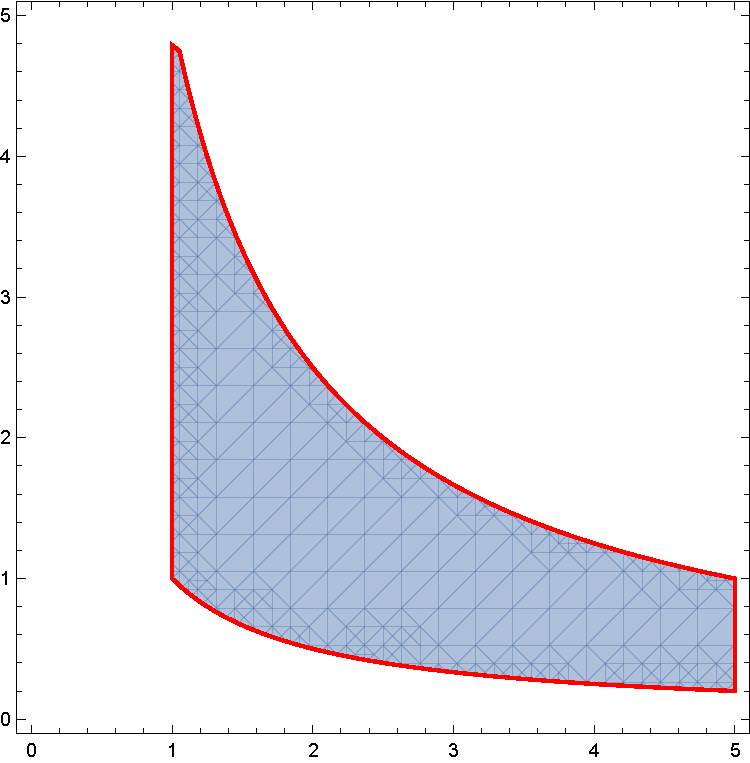
\includegraphics[scale=0.5]{p14.pdf}
\end{center}
The relations between differentials (in the region where $ u \neq 0$) are
\begin{align*}
dx & = du \\
dy & = -\frac{v}{u^2} du + \frac{1}{u} dv,
\end{align*}
therefore the area element can be expressed as 
\begin{equation*}
dA = dy \, dy = \frac{1}{u} du \, dv.
\end{equation*}
The integral is thus 
\begin{align*}
\int \int_{R} \frac{x}{1+x^2y^2} dA & = \int_{1}^{5} \int_{1}^{5} \left(\frac{u}{1+v^2}\right)\left(\frac{1}{u}\right) \, du \, dv\\
& = \int_{1}^{5} \int_{1}^{5} \left(\frac{1}{1+v^2}\right) \, du \, dv\\
& = \int_{1}^{5} \left[ \frac{u}{1+v^2} \Big|_{u=1}^{u=5} \right] \, dv \\
& = \int_{1}^{5} \frac{4}{1+v^2} \, dv \\
& = \left[4\arctan(v) \Big|_{v=1}^{v=5} \right] \\
& = 4\arctan(5)-\pi.
\end{align*}
\end{newsolution}

\end{document}

